\begin{scanpage}{0230}{212}
\begin{center}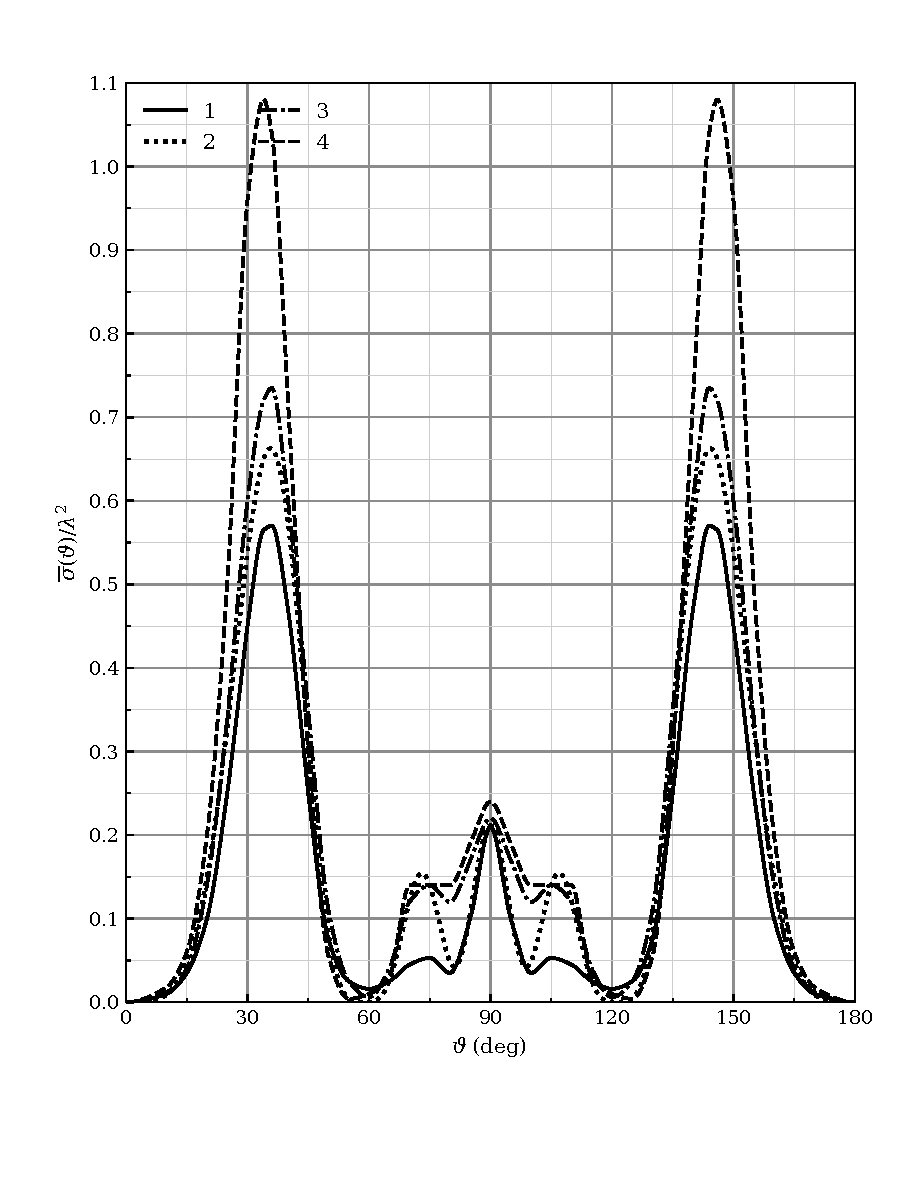
\includegraphics[width=.56\linewidth]{images/recreated/r-0230-fig80.pdf}\par
\begin{minipage}{.76\linewidth}Figure 80. Diagrams for the effective scattering area of a vibrator calculated by various methods. The designations are the same as those in Figure 79.\par\centering $L=2\lambda$\end{minipage}\end{center}
\noindent obtain the first approximation; however, its results, especially for long conductors, may depend in a substantial way on the form of the trial function. In the induced emf method [86], the current is sought in the form of a combination of trigonometric functions with unknown coefficients. These coefficients are determined by using the law of conservation of energy. This is the simplest method, but it has a number of serious defects. Thus, as a consequence of incorrectly accounting for the current component having the incident field phase,
\end{scanpage}
